\section{Modeling a Biological System }
\label{Modeling a Biological System }

This example was inspired by a paper that uses the UKF to model the biological pathway of metabolites. A metabolite is small bodily structure that is the byproduct of the metabolism. Data regarding metabolites is highly influenced by noise, which is a factor that makes other approaches, such as regression and annealing, fail. The system in the model is complex, containing 18 unknown parameters and four state variables. Initial data contained information about metabolites at various time steps \cite{article5} . \\

\noindent In the paper, researchers had access to their own data sources and used an approach that was adapted from the UKF. Though we are not using their exact dataset, we will be simulating data using the same approach as the previous example. Unlike the paper, this example will be following UKF algorithm and then comparing the result of both methods. Ultimately, the goal of this example is to demonstrate how an UKF works on higher dimensional and more complex systems, how an UKF corrects for multiple variables, and how parameters can be adjusted to fit the model. \\

\newpage

\begin{figure}[h]
    \centering
    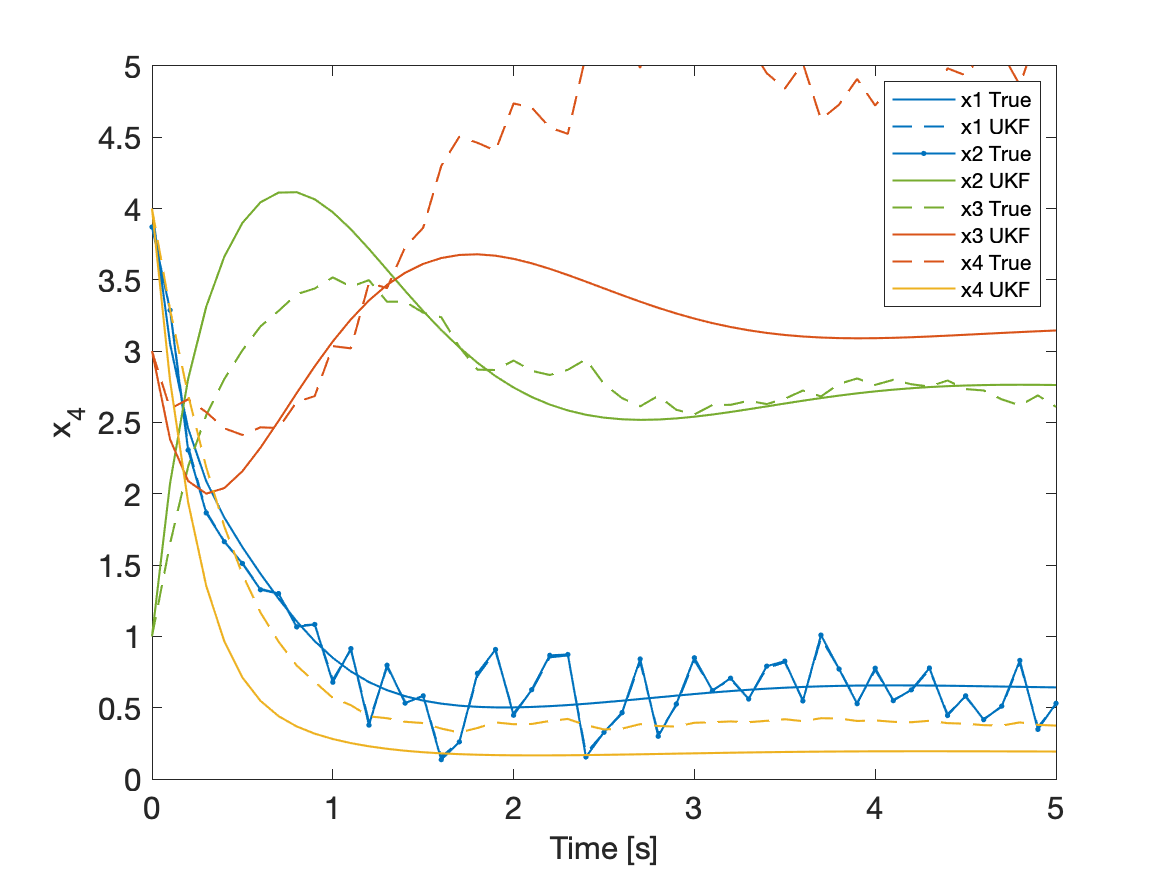
\includegraphics[scale = 0.6]{Meskin_overall.png}
    \caption{Performance of all state variables with the following conditions: R = 0.001, Q = (0.02 0.01 .03 .04) and initial values = (4, 1, 3, 4).
    Paramaters included:  }% $, \alpha = 1, \kappa = 0  }
    \label{map}
\end{figure}

\noindent Similar to the previous example, the system's true output is simulated using an ODE solver. We are given the differential equation for the four state variables. \\

\noindent The paper was able to make the model converge faster by resetting the covariance to re-excite the model. By skipping this step, the three state variables without measurements converge significantly slower.

\newpage

\begin{figure}[h]
    \centering
    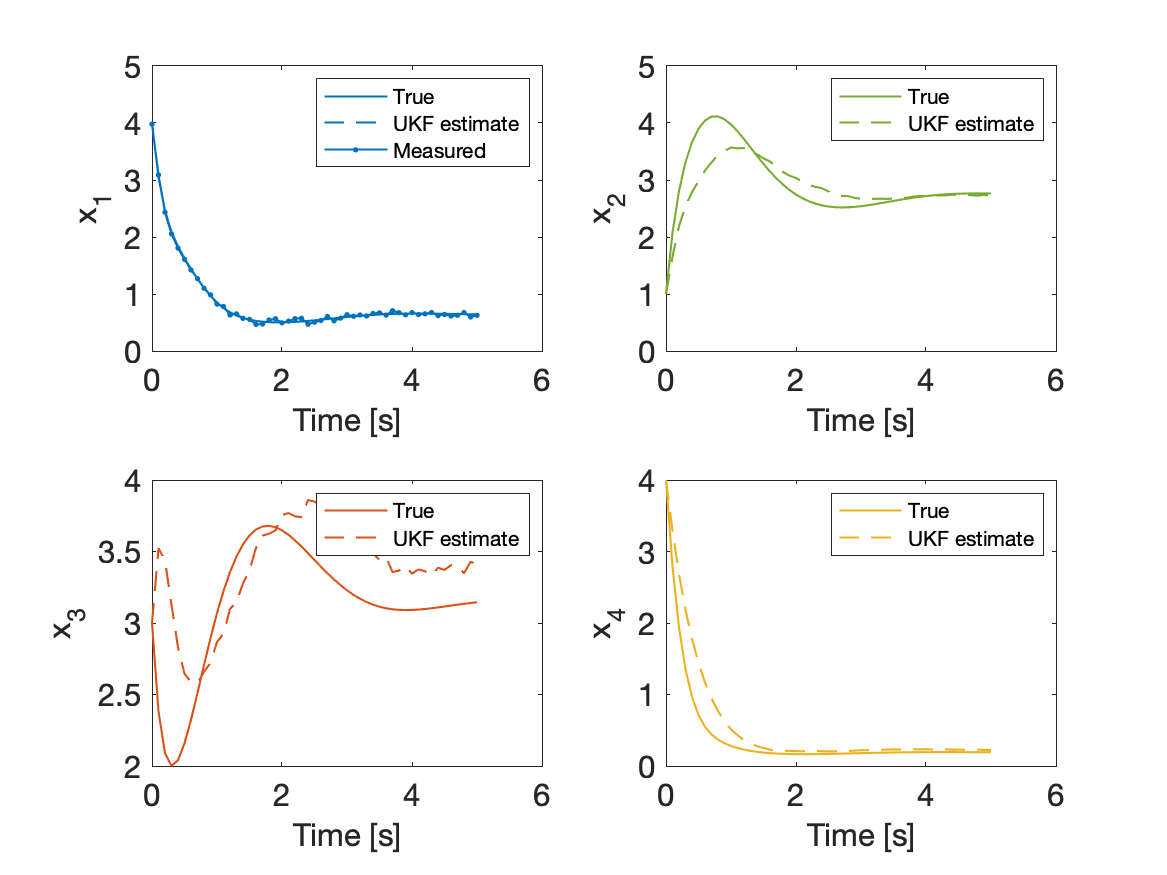
\includegraphics[scale = 0.6]{Meskin_states.png}
    \caption{Performance of all four state variables with one corrected state. The first state variable (blue) is the only one that is receiving measurements from the system. This explains why it is more accurate and converges better with the system, as compared with the other three states.}
    \label{map}
\end{figure}




\noindent \textcolor{red}{Expand here on tweaking parameters}.In theory, values of $\kappa$ can be negative, but cannot be used on MATLAB. \\


\noindent \textcolor{red}{Expand here on correcting for 1+ states}